\subsection{Remote controller}

På figur \ref{fig:ibd_remotecontroller} vises ibd til Remote controller, der består af receiver, transmitter og switch board. Blokken gør det muligt at switche mellem autonom og manuel styring. Afhængig af det signal receiver blokken modtager fra transmitter benyttes henholdsvis manuel eller autonom flyvning. Når der flyves autonom, benyttes PWM signaler fra main controller til styring, og under manuel flyvning benyttes signaler fra receiver.

\begin{figure}[H]
\centering
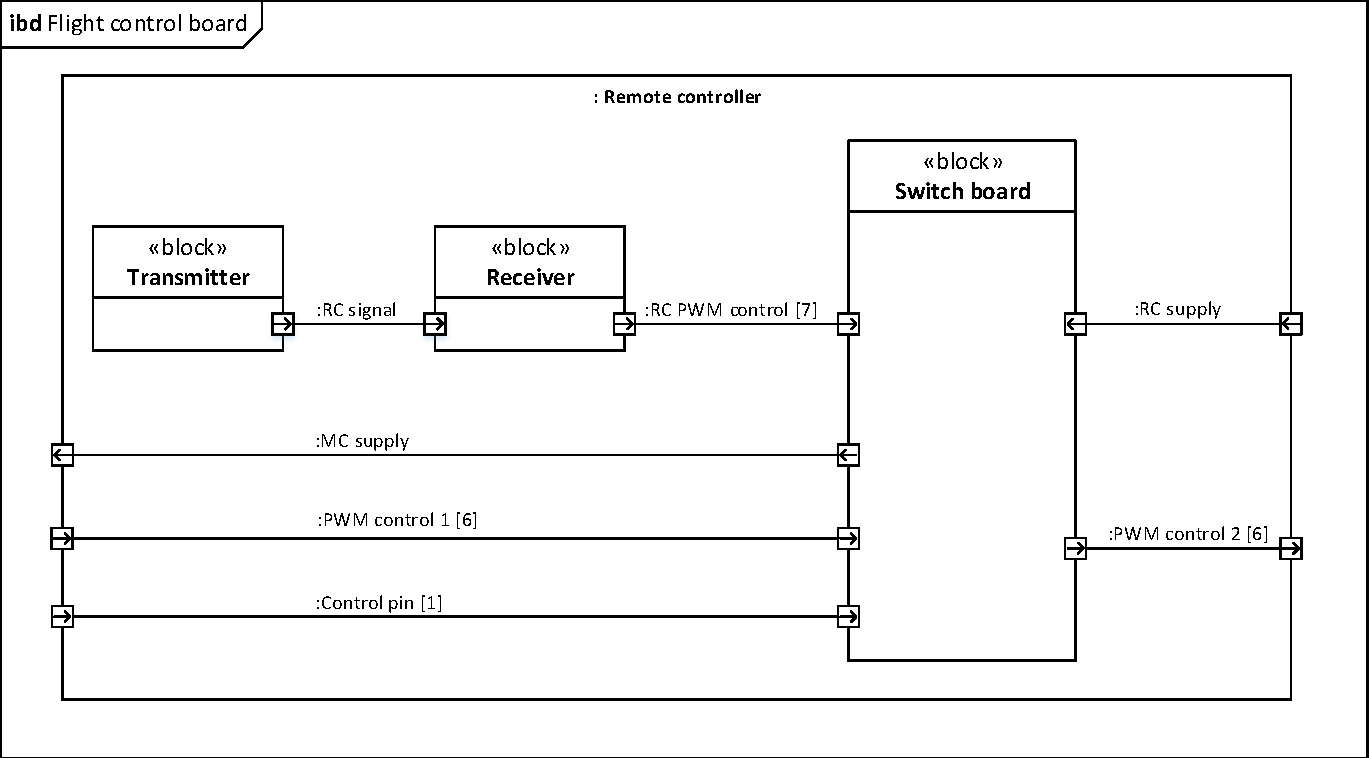
\includegraphics[width=1\textwidth]{Billeder/IBD/ibd7_remotecontroller.pdf}
\vspace{-0.5cm}
\caption{Ibd - Remote controller}
\label{fig:ibd_remotecontroller}
\end{figure}

\begin{table}[H]
	\centering
		\begin{tabular}{|p{3.5 cm}|p{4.5 cm}|p{2.6 cm}|p{2.6 cm}|} 
		\hline
			\textbf{Signal navn} 	& \textbf{Signal beskrivelse}		& \textbf{Out} 				& \textbf{In}     \\ \hline
			RC supply & 5V DC til switch board. & Flight control board. & Switch board.	\\ \hline	
			PWM control 2 [6] & 6 PWM signaler. \newline Enten 244 Hz eller 50 Hz & Switch board. & Flight control board.				\\ \hline
					
			RC PWM control [7] & 6 PWM signaler på 50 Hz \newline + GND & Reciever. & Switch board.				\\ \hline
			RC signal & 2,4 GHz trådløs \newline kommunikation & Reciever. & Switch board.				\\ \hline
			
			MC supply 			& 5V DC. 						& Switch board.  & Main controller	\\ \hline
			PWM control 1 [6] 	& 6 PWM signaler på 244 Hz. 	& Main controller & Switch board. \\ \hline
			Control pin [1]		& Skifter mellem 5V og 0V		& Main controller	& Remoto \newline  controller.    \\ \hline
		\end{tabular}
	\caption{Forbindelser til: Ibd - remote controller. }
	\label{tab:ibd_remote_controller}
\end{table}



